\documentclass[tikz,border=1.35mm]{standalone}

\definecolor{fvmadaptedge}{HTML}{8A7E7E}

\definecolor{splitred}{HTML}{AF2525}
\definecolor{splitgreen}{HTML}{0E8814}

% One quadrilateral child face highlighted inside a split irregular face.
% Coordinates are in millimeters; y=-1mm keeps the SVG-style origin at top left.
\begin{document}
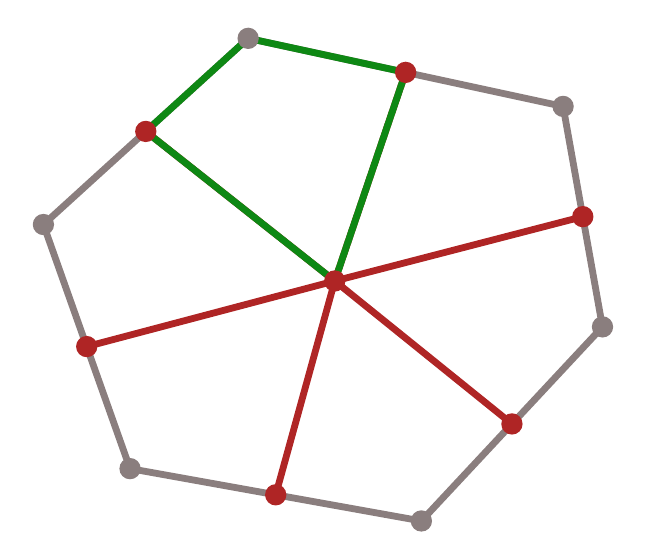
\begin{tikzpicture}[
  x=1mm,
  y=-1mm,
  line join=round,
  edge/.style={draw=fvmadaptedge,line width=0.865mm},
  splitline/.style={draw=splitred,line width=0.865mm},
  greenedge/.style={draw=splitgreen,line width=0.865mm}
]
  % Match the artwork frame before the standalone border is applied.
  \useasboundingbox (0,0) rectangle (76.000,64.000);

  % Original irregular face vertices plus split-created edge midpoints and face center.
  \coordinate (v0) at (28.000,1.353);
  \coordinate (v1) at (68.000,10.000);
  \coordinate (v2) at (73.000,38.000);
  \coordinate (v3) at (50.000,62.647);
  \coordinate (v4) at (13.000,56.000);
  \coordinate (v5) at (2.000,25.000);
  \coordinate (m01) at (48.000,5.677);
  \coordinate (m12) at (70.500,24.000);
  \coordinate (m23) at (61.500,50.324);
  \coordinate (m34) at (31.500,59.324);
  \coordinate (m45) at (7.500,40.500);
  \coordinate (m50) at (15.000,13.177);
  \coordinate (center) at (39.000,32.167);

  % Draw the boundary topology in #8a7e7e first.
  \draw[edge] (v0) -- (m01) -- (v1) -- (m12) -- (v2) -- (m23)
    -- (v3) -- (m34) -- (v4) -- (m45) -- (v5) -- (m50) -- cycle;
  \foreach \p in {m01,m12,m23,m34,m45,m50} {
    \draw[splitline] (center) -- (\p);
  }

  % Green edges indicate the selected child face near the top vertex.
  \draw[greenedge] (m50) -- (v0) -- (m01) -- (center) -- cycle;

  % Original vertices are #8a7e7e.
  \foreach \p in {v0,v1,v2,v3,v4,v5} {
    \fill[fvmadaptedge] (\p) circle[radius=1.353mm];
  }

  % Split-created edge and face nodes are red.
  \foreach \p in {m01,m12,m23,m34,m45,m50,center} {
    \fill[splitred] (\p) circle[radius=1.353mm];
  }
\end{tikzpicture}
\end{document}
